\documentclass[spanish]{article}

\usepackage[utf8]{inputenc}
\usepackage{fancyhdr} % Required for custom headers
\usepackage{lastpage} % Required to determine the last page for the footer
\usepackage{extramarks} % Required for headers and footers
\usepackage{amssymb}
\usepackage{amsmath}
\usepackage{mathtools}
%\usepackage{graphicx} % Required to insert images
\usepackage{babel}
%\usepackage{url}
\usepackage{tikz}
\usepackage{tabto}

\usetikzlibrary{automata,positioning}
\usetikzlibrary{babel}

\def\e{\varepsilon}
\def\ra{\rightarrow}


\newcommand{\me}{Gabriel De La Parra}
\newcommand{\class}{CC3102 - Teoría de la Computación}
\newcommand{\institution}{Departamento de Ciencias de la Computación\\ \textsc{Universidad de Chile}}
\newcommand{\task}{Tarea 2: Lenguajes libres de contexto y máquinas de Turing}

\topmargin=-.45in
\evensidemargin=0in
\oddsidemargin=0in
\textwidth=6.5in
\textheight=9.0in
\headsep=0.25in


\pagestyle{fancy}
\lhead{\me} % Top left header
\rhead{\task} % Top right header
\cfoot{} % Bottom center footer
\rfoot{\thepage\ / \protect\pageref{LastPage}} % Bottom right footer

% Title Page
\title{\task \\ {\normalsize \class \\ \institution \\}}

\author{\me}
\date{\today}


\begin{document}
\maketitle
\newpage
\tableofcontents
\newpage

\section{Problema 1}
\textbf{Entregue los diagramas de estados de los autómatas de pila que reconocen los siguientes lenguajes. Adjunte también una descripción intuitiva y de alto nivel de cómo opera el autómata de pila.}
\\\\
$(a)$. $L_1 = \{x_1\#x_2\#...\#x_k | k\geq1$, cada $x_i\in\{a,b\}^*$, y existen i, j tales que $x_i=x_j^R\}$
\\\\
Para que un AP pueda reconocer el lenguaje propuesto, debe hacerse uso del no-determinismo. La idea central es que $A_1$, el autómata que reconoce $L_1$, pueda ``elegir'' un $x_i$ para guardar en la pila, y un $x_j$ para compararlo. Gracias al no-determinismo, se pueden considerar así todos los $x_i$.
\\\\
Para guardar un $x_i$ el autómata puede recorrer $\{a,b,\#\}^*$ elementos. Las transiciones de entrada hacia el estado $q_{save}$ están precedidas por un $\#$, por lo que se puede empezar a guardar solo después de éste símbolo, salvo el caso inicial $x_1$, donde no hay $\#$. Posteriormente, se puede avanzar, bajo el mismo principio, hasta encontrar otro grupo $x_j$ y realizar la comparación. 
\\\\
La comparación, que se realiza en $q_{cmpr}$, es positiva cuando se saca todo lo que se metió a la pila de $A_1$ y queda solo el símbolo $\$$, insertado al inicio, para denotar el final de la pila. Debe considerarse que, posterior a vaciar la pila, puede ser necesario avanzar hasta el final de la entrada, sobre otros $x_k$ hasta llegar al final.
\\\\
Se debe considerar adicionalmente el caso donde k=1 o i=j. En tal caso, no hay símbolo $\#$ y la palabra debe ser palíndrome. En tal caso, se agrega un estado $q_{strt}$, en el cual se guardan los símbolos iniciales de la palabra y posteriormente se debe sacar en $q_{end}$. Si la pila queda vacía al final de recorrer la entrada, se acepta. No se considera el caso de la palabra impar, sin embargo ya se ha visto anteriormente, que corresponde a no-deterministicamente saltarse el símbolo central.
\\\\
Se presenta a continuación una descripción de alto nivel:
\begin{itemize}
\item Colocar un símbolo para denotar el inicio de la pila;
\item Elegir una palabra $x_i$;
\item Guardar todos los símbolos de la palabra $x_i$ en la pila;
\item Elegir una palabra $x_j$;
\item Por cada símbolo de $x_j$ sacar el mismo símbolo de la pila;
\item Si se llega al final de la palabra y se llega al símbolo de inicio de la pila, acepta, de lo contrario rechaza;
\end{itemize}
El diagrama de estados para el autómata está dado por la siguiente figura:
\begin{center}
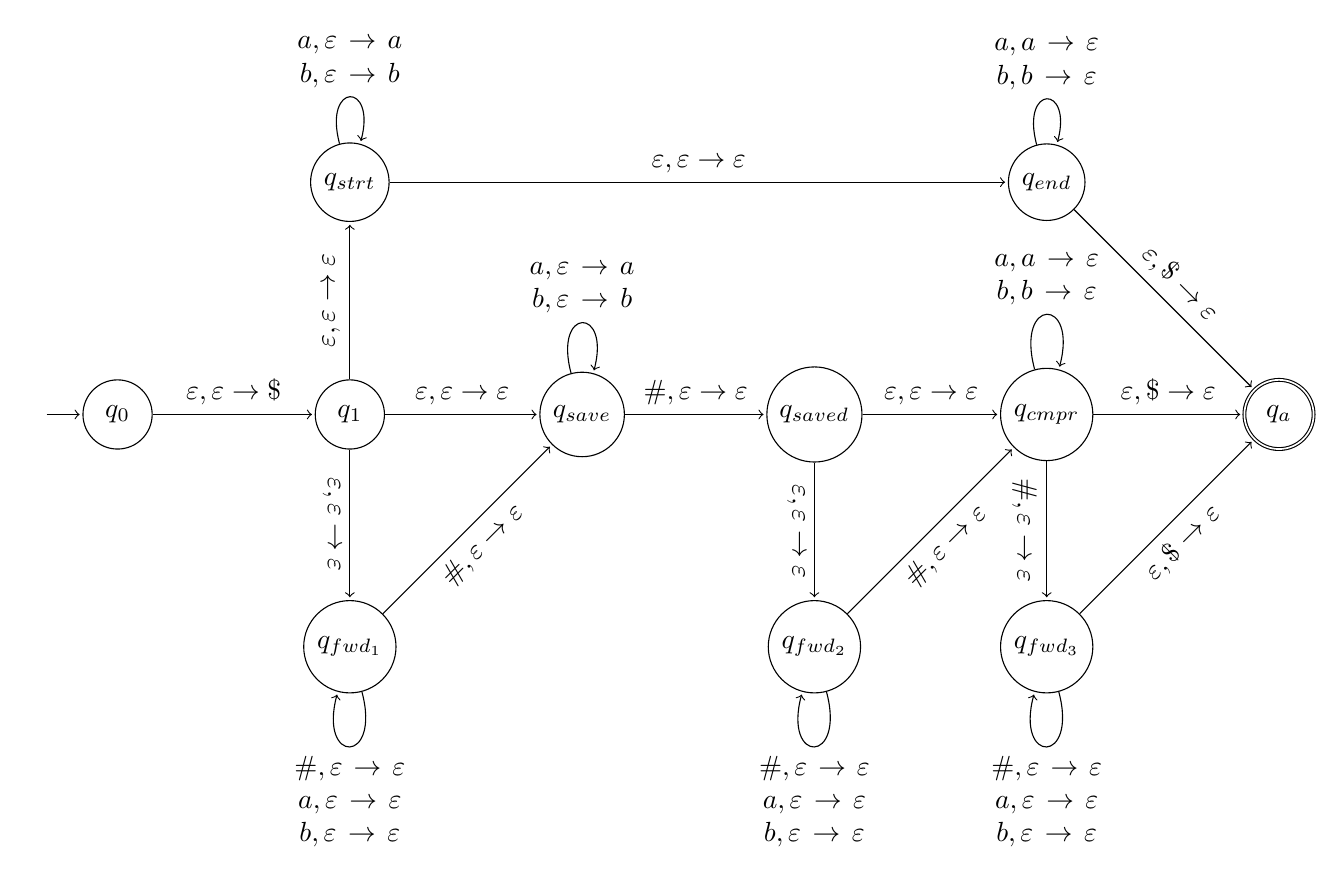
\begin{tikzpicture}[shorten >=1pt,node distance=2.95cm,on grid,auto]
\node[state,initial, initial text={}]	(q_0)									{$q_0$}; 
\node[state]							(q_01)		[right=of q_0]				{$q_1$}; 
\node[state]							(q_save)	[right=of q_01]				{$q_{save}$}; 
\node[state]							(q_fwd1)	[below=of q_01]				{$q_{fwd_1}$}; 
\node[state]							(q_saved)	[right=of q_save]			{$q_{saved}$};	
\node[state]							(q_cmpr)	[right=of q_saved]			{$q_{cmpr}$}; 
\node[state]							(q_fwd2)	[below=of q_saved]			{$q_{fwd_2}$};
\node[state,accepting]					(q_f)		[right=of q_cmpr]			{$q_a$};
\node[state]							(q_fwd3)	[below=of q_cmpr]			{$q_{fwd_3}$};

\node[state]							(q_2)		[above=of q_01]				{$q_{strt}$}; 
\node[state]							(q_3)		[above=of q_cmpr]			{$q_{end}$};
\path[->] 

(q_01)		edge					node[sloped, anchor=center, above]			{$\e,\e\ra\e$}								(q_2)
(q_2)		edge	[loop above]	node[text width=2cm,align=center]			{$a,\e\ra a$\\$b,\e\ra b$}					()
			edge					node[sloped, anchor=center, above]			{$\e,\e\ra\e$}								(q_3)
(q_3)		edge	[loop above]	node[text width=2cm,align=center]			{$a,a\ra\e$\\$b,b\ra\e$}					()
			edge					node[sloped, anchor=center, above]			{$\e,\$\ra\e$}								(q_f)

(q_0)		edge					node										{$\e,\e\ra\$$}								(q_01)

(q_01)		edge					node										{$\e,\e\ra\e$}								(q_save)
			edge					node[sloped, anchor=center, below]			{$\e,\e\ra\e$}								(q_fwd1)
		
(q_save)	edge					node										{$\#,\e\ra\e$}								(q_saved)
			edge	[loop above]	node[text width=2cm,align=center]			{$a,\e\ra a$\\$b,\e\ra b$}					()
		
(q_fwd1)	edge					node[sloped, anchor=center, below]			{$\#,\e\ra\e$}								(q_save)
			edge	[loop below]	node[text width=2cm,align=center]			{$\#,\e\ra\e$\\$a,\e\ra\e$\\$b,\e\ra\e$}	()

(q_saved)	edge					node										{$\e,\e\ra\e$}								(q_cmpr)
			edge					node[sloped, anchor=center, below]			{$\e,\e\ra\e$}								(q_fwd2)				
			
(q_cmpr)	edge					node										{$\e,\$\ra\e$}								(q_f)
			edge	[loop above]	node[text width=2cm,align=center]			{$a,a\ra\e$\\$b,b\ra\e$}					()
			edge					node[swap, sloped, anchor=center, below]	{$\#,\e\ra\e$}								(q_fwd3)
				
(q_fwd2)	edge					node[sloped, anchor=center, below]			{$\#,\e\ra\e$}								(q_cmpr)
			edge	[loop below]	node[text width=2cm,align=center]			{$\#,\e\ra\e$\\$a,\e\ra\e$\\$b,\e\ra\e$}	()	
			
(q_fwd3)	edge					node[sloped, anchor=center, below]			{$\e,\$\ra\e$}								(q_f)
			edge	[loop below]	node[text width=2cm,align=center]			{$\#,\e\ra\e$\\$a,\e\ra\e$\\$b,\e\ra\e$}	()				
;
\end{tikzpicture}
\end{center}
\newpage
$(b)$. $L_2=\{w\in\{a,b\}*|\|w\|_a=2*\|w\|_b\}$, donde $\|w\|_x$ es el número de veces que aparece el símbolo $x\in \{a,b\}$ en $w$.
\\\\
Las palabras dentro de $L_2$ son todas aquellas que tengan el doble de $b's$ que $a's$. Para encontrar las palabras dentro del lenguaje se utiliza la misma idea del autómata que compara que la cantidad de $a's$ y $b's$ sean iguales. Este autómata utiliza la pila para guardar la referencia de comparación de $a's$ y $b's$, es decir, si se han leído $n$ $a's$ más que $b's$, la pila tendrá $n$ $a's$. En el caso contrario, el autómata guardará $n$ $b's$. El autómata acepta si cuando se procesa toda la cadena, el símbolo de tope $(\$)$ de la pila se procesa. 
\\\\
La adaptación a nuestro problema consiste en que por cada $a$ que se lee, se deben agregar dos $a's$, para compensar que sean el doble de $b's$. Las condiciones de aceptación son las mismas.
\\\\
Se presenta a continuación una descripción de alto nivel:
\begin{itemize}
\NumTabs{30}
\item Colocar un símbolo $\$$ para denotar el inicio de la pila;
\item Si se lee una $a$;
\item \tab Si al hacer pop, la pila tiene $\$$, colocar $\$$ y colocar 2x$a$, continuar;
\item \tab Si al hacer pop, la pila tiene $a$, colocar 3x$a$, una por la que se hizo pop, y dos más, continuar;
\item \tab Si al hacer pop, la pila tiene $b$, continuar;
\item Si se lee una $b$;
\item \tab Si al hacer pop, la pila tiene $\$$, colocar $\$$ y colocar $b$, continuar;
\item \tab Si al hacer pop, la pila tiene $b$, colocar 2x$b$, una por la que se hizo pop, y una más, continuar;
\item \tab Si al hacer pop, la pila tiene $a$, continuar;
\item Si se llega al final de la palabra y se llega al símbolo de inicio de la pila, acepta, de lo contrario rechaza;
\end{itemize}
El diagrama de estados para el autómata está dado por la siguiente figura:
\begin{center}
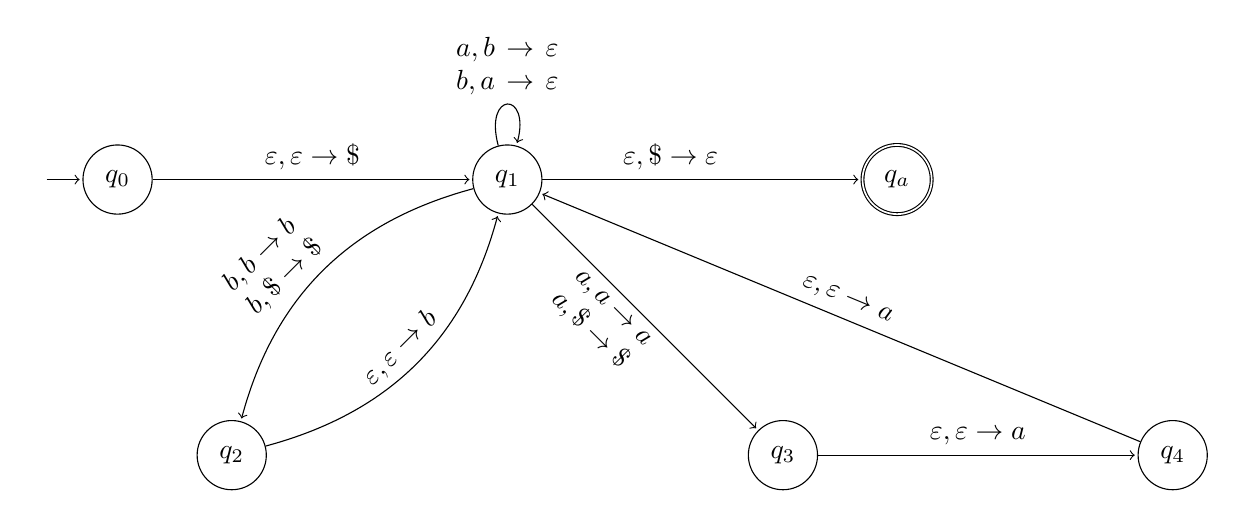
\begin{tikzpicture}[shorten >=1pt,node distance=4.95cm,on grid,auto]
\node[state,initial, initial text={}]	(q_0)											{$q_0$};
\node[state]							(q_1)		[right=of q_0]						{$q_1$}; 
\node[state]							(q_2)		[below left=of q_1]					{$q_2$}; 
\node[state]							(q_3)		[below right=of q_1]				{$q_3$}; 
\node[state]							(q_4)		[right=of q_3]						{$q_4$}; 
\node[state,accepting]					(q_f)		[right=of q_1]						{$q_a$}; 
\path[->] 
(q_0)		edge					node												{$\e,\e\ra\$$}								(q_1)

(q_1)		edge	[loop above]	node[text width=2cm,align=center]					{$a,b\ra\e$\\$b,a\ra\e$}					()
			edge					node[text width=2cm, anchor=center,above,sloped]	{$\e,\$\ra\e$}								(q_f)
			edge	[bend right]	node[text width=2cm, anchor=center,above,sloped]	{$b,b \ra b$\\$b,\$\ra \$$}					(q_2)
			edge					node[text width=2cm, anchor=center,below,sloped]	{$a,a \ra a$\\$a,\$\ra \$$}					(q_3)				
	
(q_2)		edge	[bend right]	node[sloped, anchor=center, above]					{$\e,\e\ra b$}								(q_1)	

(q_3)		edge					node[sloped, anchor=center, above]					{$\e,\e\ra a$}								(q_4)

(q_4)		edge					node[sloped, anchor=center, above]					{$\e,\e\ra a$}								(q_1)				
;
\end{tikzpicture}
\end{center}
\newpage
\section{Problema 2}
\textbf{Mostrar usando el lema de bombeo que los siguientes lenguajes no son libres de contexto.}
\\\\
$(a)$. $L_3$ es el conjunto de las cadenas formadas por símbolos $a$, $b$ y $c$ con misma cantidad de $a$, $b$ y $c$. Ejemplo: $abcabc$, $abbcaccab$, $bcaaacbcb$, ...
\\\\
La palabra $a^nb^nc^n$ pertenece al lenguaje. Se ha demostrado en cátedra, que esta palabra al ser bombeada, no pertenece a los lenguajes libres de contexto.
\\\\
Sea $s=a^pb^pc^p$, donde el largo de la palabra, tal que $|s|=3\geq p$. \\
Se deben considerar las posibles particiones para $uv^ixy^iz$, que satisfagan las condiciones del bombeo:
\begin{itemize}
\item $\forall i \geq 0$ para $uv^ixy^iz \in L_3$ 
\item $|vy|>0$
\item $|vxy|\leq 0$
\end{itemize}
Las posibilidades se reducen a que $vxy$ se compone de un solo símbolo o se compone de dos.
\begin{itemize}
\item Si $v$ o $y$ se componen de dos símbolos ($ab$ o $bc$), al ser bombeado, genera estructuras del tipo $abab$ o $bcbc$, las cuales rompen la estructura de la palabra. $\therefore \notin L_3$
\item Si $v$ o $y$ se componen de un solo símbolo, basta bombear a $0$ o $2$ para que se haga una desigualdad entre los dos símbolos bombeados y el no bombeado. $\therefore \notin L_3$
\end{itemize}
$(b)$. $L_4 = {a^nb^nc^m : n \leq m \leq 2n}$
\\\\
La palabra vista anteriormente, $a^nb^nc^n$ también pertenece a este lenguaje. La demostración es la misma que en el caso anterior.
\newpage
\section{Problema 3}
$(b)$.  Considere la siguiente gramática $G: S \ra XY , X \ra aXb | \e, Y \ra bYa | \e$. Describa en forma concisa (en Castellano o con una fórmula corta) el lenguaje generado por la gramática. Convierta la gramática anterior $G$ a la Forma Normal de Chomsky.
\\\\
El lenguaje genera todas las palabras de la forma:
\begin{center}
$L_G=\{a^nb^{n+m}a^m$ $|$ $n,m \geq 0\}$
\end{center}
La conversión a la forma normal de Chomsky implica que todas las reglas cumplan los siguientes criterios:
\\\\
a. El símbolo inicial puede derivar una sola vez.\\
b. Las variables pueden ir a dos variables o un terminal, es decir $A \ra BC$ o $A \ra a$. 
\\\\
Inicialmente se agrega una nueva regla para la variable inicial $S_0$. Si bien este paso se encuentra dentro del procedimiento, la regla S no está en la derivación de ninguna otra regla, por lo que S quedaría como una transición inalcanzable. Se elimina esta derivación adicional.
\begin{center}
$S \ra XY$\\
$X \ra aXb | \e$\\
$Y \ra bYa | \e$
\end{center}
El procedimiento de conversión implica reemplazar todas las reglas $\ra \e$: $Y \ra \e$ y $X \ra \e$:
\begin{center}
$S \ra XY|X|Y$\\
$X \ra aXb|ab$\\
$Y \ra bYa|ba$
\end{center}
Luego es necesario reemplazar las reglas que son uno a uno en variable: $S \ra X$, $S \ra Y$:
\begin{center}
$S \ra XY|aXb|ab|bYa|ba$\\
$X \ra aXb|ab$\\
$Y \ra bYa|ba$
\end{center}
Se agregan reglas para convertir a la FNC:
\begin{center}
$A \ra a$\\
$B \ra b$
\end{center}
Al sustituir, queda:
\begin{center}
$S \ra XY|aXb|bYa|AB|BA$\\
$X \ra aXb|AB$\\
$Y \ra bYa|BA$\\
$A \ra a$\\
$B \ra b$
\end{center}
Adicionalmente se agregan dos reglas más:
\begin{center}
$U \ra AX$\\
$V \ra BY$
\end{center}
Finalmente, la gramática queda en la FNC definida por las siguientes reglas:
\begin{center}
$S \ra XY|UB|VA|AB|BA$\\
$X \ra UB|AB$\\
$Y \ra VA|BA$\\
$U \ra AX$\\
$V \ra BY$\\
$A \ra a$\\
$B \ra b$
\end{center}
\newpage
\section{Problema 4}
Un autómata de cola (AC) se define de manera análoga a un autómata de pila, pero usando una cola. Recuerde que una cola es una estructura de datos con memoria ilimitada donde por un extremo se puede sólo insertar elementos y por el otro extremo sólo poner elementos.
\\\\
(a). Entregue una definición formal de un AC, incluyendo qué significa que un AC acepte una palabra.
\\\\
(b). Demuestre que un AC es equivalente en poder a una Máquina de Turing.
\\\\
De manera general, un autómata de cola puede almacenar símbolos de tal forma que el último símbolo que se agrega, es el último que se saca (o alternativamente, el primero que se introduce, es el primero que sale). 
\\\\
Esta capacidad, de poder sacar el primer elemento y colocarlo al final, se puede explotar de tal forma que al repetir varias veces, es posible rotar los elementos almacenados en la cola. Al poder rotar sobre sus elementos almacenados, es posible no solo moverse de izquierda a derecha, sino también simular el movimiento de derecha a izquierda, al rotar en $n-1$ la cola de tamaño $n$, pudiendo agregar algún símbolo especial para denotar la el inicio y fin de la cola.
\\\\
Si se considera que se podría almacenar el $input$, le daría también la capacidad de poder modificar su entrada. Adicionalmente, el rotar le permite agregar $\sqcup$ a medida que agrega nuevos símbolos. Más aún, se puede extender a que se agregue un símbolo adicional para demarcar la posición del cabezal. Se podrían incluso implementar movimientos de desplazamiento (shift left/right).De todo lo anterior, la semejanza con una máquina de Turing. 
\\\\
La equivalencia en sentido contrario, es que una máquina de Turing puede mover el cabezal, permitiendo programar que introducir o remover elementos tenga que realizarse en cierto orden LILO o FIFO, como el de una cola. De esta forma, se podría tener la entrada en una parte de la cinta y en otra parte, separadas por algún símbolo especial, la cola. Lo mismo se vió anteriormente cuando se mencionaron las MT multicinta. En tal caso, se tendría una cinta para la entrada y una cinta para la cola.
\\\\
La definición formal está dada por una 6-tupla $(Q, \Sigma, \Gamma, \delta, q_0, F)$, similar a la de un autómata de pila. La principal diferencia se encuentra en la forma en que se introducen y extraen los elementos.
\begin{itemize}
\item $Q$: Conjunto de estados;
\item $\Sigma$: Alfabeto de entrada;
\item $\Gamma$: Alfabeto de la cola;
\item $\delta$: Función de transición: En un estado determinado, lee un símbolo de la entrada, saca un símbolo de la cola, agrega un símbolo a la cola y se mueve al siguiente estado;
\item $q_0$: Estado inicial;
\item $F \subseteq Q$: Conjunto de estados finales;
\end{itemize}
Un autómata de cola puede aceptar una palabra $w \in \Sigma$ si, existe una secuencia de transiciones, que permiten al autómata pasar del estado inicial $q_0$ a un estado final $\in F$, al leer la palabra completa y tener la cola vacía.
\newpage
\section{Problema 5}
\textbf{Entregue las MTs multicinta (descripción de alto nivel y diagramas de estados) que reconocen los siguientes lenguajes:}
\\\\
$(a)$. $L_3 = \{a^nb^mc^{min\{n,m\}}$ $|$ $n,m \geq 0 \}$
\\\\
La máquina multicinta, tiene las siguientes cintas:
\\\\
$I$: Cinta de entrada\\
$A$: Cinta para símbolos $a$\\
$B$: Cinta para símbolos $b$
\\\\
La máquina multicinta que reconoce el lenguaje, realiza de manera intuitiva lo siguiente:
\\\\
Copia las $a$ a $A$ y $b$ a $B$. Si en $I$ lee una $c$, debe leer una $a$ y una $b$, de lo contrario rechaza. Si lee un $\sqcup$ en $I$ debe leer un $\sqcup$ en $A$ y/o en $B$, de lo contrario rechaza.
\\\\
En una descripción de alto nivel, realiza lo siguiente:
\begin{itemize}
\NumTabs{30}
\item Copia, desde $I$ hasta encontrar un $b$, todos los símbolos $a$ a $A$ y mueve el cabezal al principio de $A$, dado por un $\$$.
\item Copia, desde $I$ hasta encontrar un $c$, todos los símbolos $b$ a $B$ y mueve el cabezal al principio de $B$, dado por un $\$$.
\item Desde la cinta $I$ para cada $c$ realiza la siguiente acción:
\item \tab Si lee una $c$ en $I$,
\item \tab \tab Si lee un $\sqcup$ en $A$, rechaza; 
\item \tab \tab Si lee un $\sqcup$ en $B$, rechaza; 
\item \tab \tab Si lee una $a$ en $A$, continúa.
\item \tab \tab Si lee una $b$ en $B$, continúa.
\item \tab Si lee un $\sqcup$ en $I$
\item \tab \tab Si lee un $\sqcup$ en $A$, acepta.
\item \tab \tab Si lee un $\sqcup$ en $B$, acepta.
\item \tab \tab Si lee una $a$ en $A$, rechaza.
\item \tab \tab Si lee una $b$ en $B$, rechaza.
\end{itemize}
En el diagrama de estados, por presentación, se ha separado en 2 diagramas. Un primer diagrama para guardar los valores en las dos cintas $A$, $B$.
\begin{center}
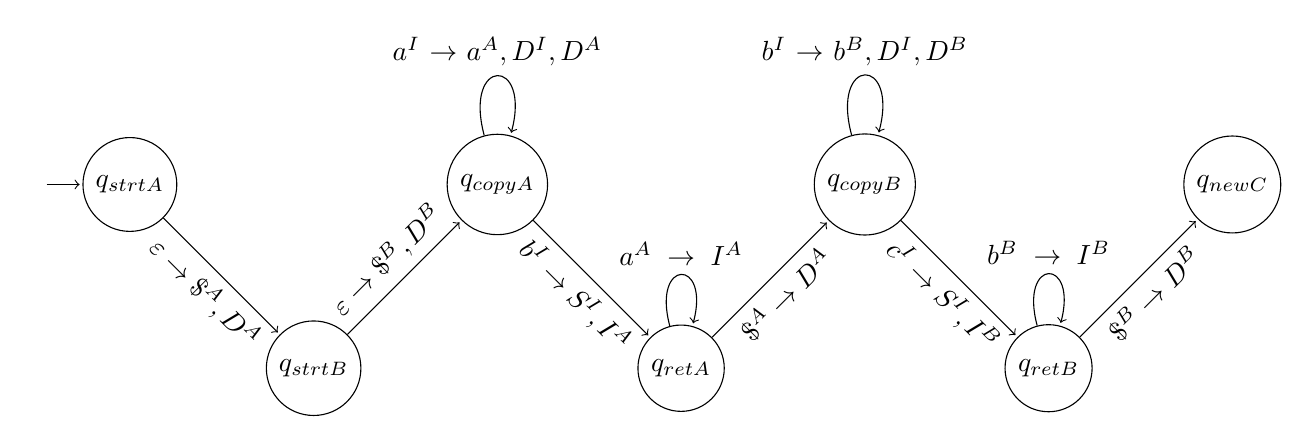
\begin{tikzpicture}[shorten >=1pt,node distance=3.3cm,on grid,auto]
\node[state,initial, initial text={}]	(q_00)											{$q_{strtA}$};
\node[state]							(q_01)		[below right=of q_00]				{$q_{strtB}$};
\node[state]							(q_1)		[above right=of q_01]				{$q_{copyA}$}; 
\node[state]							(q_2)		[below right=of q_1]				{$q_{retA}$}; 
\node[state]							(q_3)		[above right=of q_2]				{$q_{copyB}$}; 
\node[state]							(q_4)		[below right=of q_3]				{$q_{retB}$}; 
\node[state]							(q_f)		[above right=of q_4]				{$q_{newC}$}; 
\path[->] 
(q_00)		edge					node[sloped, anchor=center, below]					{$\e \ra \$^A,D^A$}							(q_01)

(q_01)		edge					node[sloped, anchor=center, above]					{$\e \ra \$^B,D^B$}							(q_1)

(q_1)		edge	[loop above]	node[text width=3cm, align=center]					{$a^I \ra a^A,D^I,D^A$}						()		
			edge					node[anchor=center, below, sloped]					{$b^I \ra S^I,I^A$}						(q_2)
			
(q_2)		edge	[loop above]	node[text width=3cm, align=center]					{$a^A \ra I^A$}								()		
			edge					node[anchor=center, below, sloped]					{$\$^A \ra D^A$}							(q_3)

(q_3)		edge	[loop above]	node[text width=3cm, align=center]					{$b^I \ra b^B,D^I,D^B$}						()		
			edge					node[anchor=center, below, sloped]					{$c^I \ra S^I,I^B$}							(q_4)

(q_4)		edge	[loop above]	node[text width=3cm, align=center]					{$b^B \ra I^B$}								()		
			edge					node[anchor=center, below, sloped]					{$\$^B \ra D^B$}							(q_f)
;
\end{tikzpicture}
\end{center}
Se presenta la segunda parte, el diagrama para procesar $c$. La transición final desde $q_{noC}$ puede llegar a un estado de aceptación y rechazo por el no-determinismo. Si existiera algún conflicto por estas transiciones, habría que modificar el diagrama para que revise en primera instancia los $\sqcup$ y posteriormente los símbolos, como fue descrito en la descripción de alto nivel.
\begin{center}
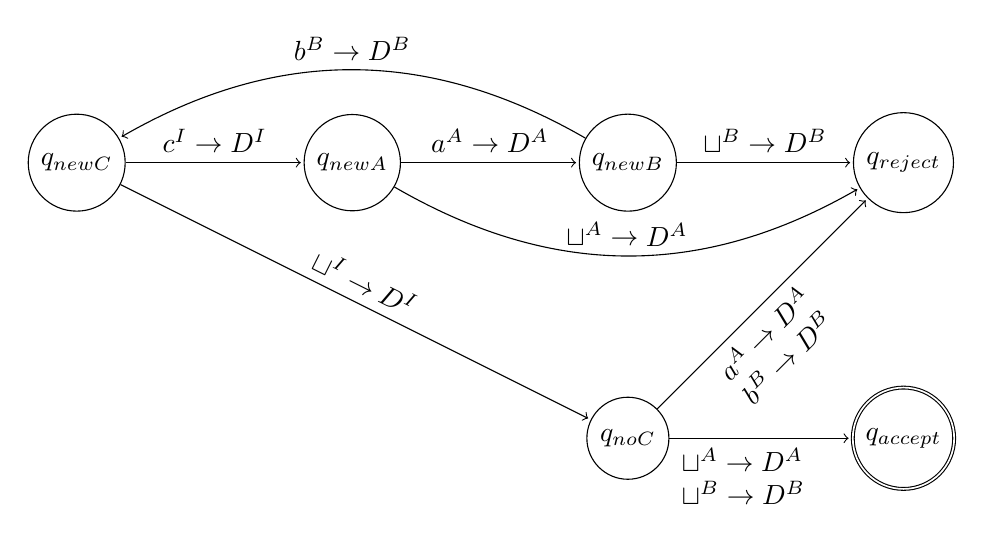
\begin{tikzpicture}[shorten >=1pt,node distance=3.5cm,on grid,auto]
\node[state]							(q_0)											{$q_{newC}$};
\node[state]							(q_1)		[right=of q_0]						{$q_{newA}$};
\node[state]							(q_2)		[right=of q_1]						{$q_{newB}$}; 
\node[state]							(q_r)		[right=of q_2]						{$q_{reject}$}; 		
\node[state,accepting]					(q_f)		[below=of q_r]						{$q_{accept}$}; 
\node[state]							(q_3)		[left=of q_f]						{$q_{noC}$}; 
\path[->] 
(q_0)		edge					node[sloped, anchor=center, above]					{$c^I \ra D^I$}								(q_1)
			edge					node[sloped, anchor=center, above]					{$\sqcup^I \ra D^I$}						(q_3)
			
(q_1)		edge					node[sloped, anchor=center, above]					{$a^A \ra D^A$}								(q_2)
			edge[bend right]		node[sloped, anchor=center, above]					{$\sqcup^A \ra D^A$}						(q_r)	
			
(q_2)		edge[bend right]		node[sloped, anchor=center, above]					{$b^B \ra D^B$}								(q_0)
			edge 					node[sloped, anchor=center, above]					{$\sqcup^B \ra D^B$}						(q_r)	

(q_3)		edge					node[text width=2cm, sloped, anchor=center, below]	{$a^A \ra D^A$\\$b^B \ra D^B$}				(q_r)	
			edge					node[text width=2cm, sloped, anchor=center, below]	{$\sqcup^A \ra D^A$\\$\sqcup^B \ra D^B$}	(q_f)
;
\end{tikzpicture}
\end{center}
\newpage
$(b)$. $L_4 = \{x\#y\#z$ $|$ $x,y,z \in \{0,1\}^*, |x|=|y|,z = x \oplus y \}$ donde $\oplus$ es el XOR binario.
\\\\
La máquina multicinta, tiene las siguientes cintas:
\\\\
$I$: Cinta de entrada\\
$X$: Cinta para símbolos de $x$\\
$Y$: Cinta para símbolos de $y$
\\\\
Intuitivamente, la máquina copia la entrada $x$ a $X$, pasa el primer $\#$, copia $y$ a $Y$, pasa el segundo $\#$ y finalmente empieza a procesar el contenido de $z$. Si $z_i$ es $0$, $x_i$ e $y_i$ deben ser distintos. Si $z_i$ es $1$, $x_i$ e $y_i$ deben ser iguales. Si en algún momento alguna de las cintas $X$ e $Y$ tienen un $\sqcup$, luego de haber leído un símbolo $z_j$, se rechaza. Si en cambio, al leer un $z_j$ las otras dos cintas no son vacío, debe rechazar. La máquina acepta cuando se cumplen los criterios anteriores.
\\\\
En una descripción de alto nivel, la máquina realiza la siguiente tarea:
\begin{itemize}
\NumTabs{30}
\item Copia, desde $I$ hasta un $\#$, todos los símbolos de $x$ a $X$ y mueve el cabezal al principio de $X$.
\item Copia, desde $I$ hasta un $\#$, todos los símbolos de $y$ a $Y$ y mueve el cabezal al principio de $Y$.
\item Desde la cinta $I$ para cada símbolo en $z$ realiza la siguiente acción:
\item \tab Si lee un $z_i = 0$ en $I$,
\item \tab \tab Si lee un $\sqcup$ en $X$, rechaza.
\item \tab \tab Si lee un $\sqcup$ en $Y$, rechaza.
\item \tab \tab Si lee un $x_i = 0$ en $X$,
\item \tab \tab \tab Si lee un $y_i = 0$ en $Y$, rechaza.
\item \tab \tab \tab Si lee un $y_i = 1$ en $Y$, continúa.
\item \tab \tab Si lee un $x_i = 1$ en $X$,
\item \tab \tab \tab Si lee un $0$ en $Y$, continúa.
\item \tab \tab \tab Si lee un $1$ en $Y$, rechaza.
\item \tab Si lee un $z_i = 1$ en $I$,
\item \tab \tab Si lee un $\sqcup$ en $X$, rechaza.
\item \tab \tab Si lee un $\sqcup$ en $Y$, rechaza.
\item \tab \tab Si lee un $x_i = 0$ en $X$,
\item \tab \tab \tab Si lee un $y_i = 0$ en $Y$, continúa.
\item \tab \tab \tab Si lee un $y_i = 1$ en $Y$, rechaza.
\item \tab \tab Si lee un $x_i = 1$ en $X$,
\item \tab \tab \tab Si lee un $0$ en $Y$, rechaza.
\item \tab \tab \tab Si lee un $1$ en $Y$, continúa.
\item \tab Si lee un $\sqcup$ en $I$,
\item \tab \tab Si lee un $x_i = 0$ en $X$, rechaza.
\item \tab \tab Si lee un $x_i = 1$ en $X$, rechaza.
\item \tab \tab Si lee un $y_i = 0$ en $Y$, rechaza.
\item \tab \tab Si lee un $y_i = 1$ en $Y$, rechaza.
\item \tab \tab Si lee un $\sqcup$ en $X$, continúa.
\item \tab \tab \tab Si lee un $\sqcup$ en $Y$, acepta.
\end{itemize}
El diagrama de estados, al igual que en $(a)$ tiene una etapa de almacenamiento de los valores en las cintas $X$ e $Y$.
\begin{center}
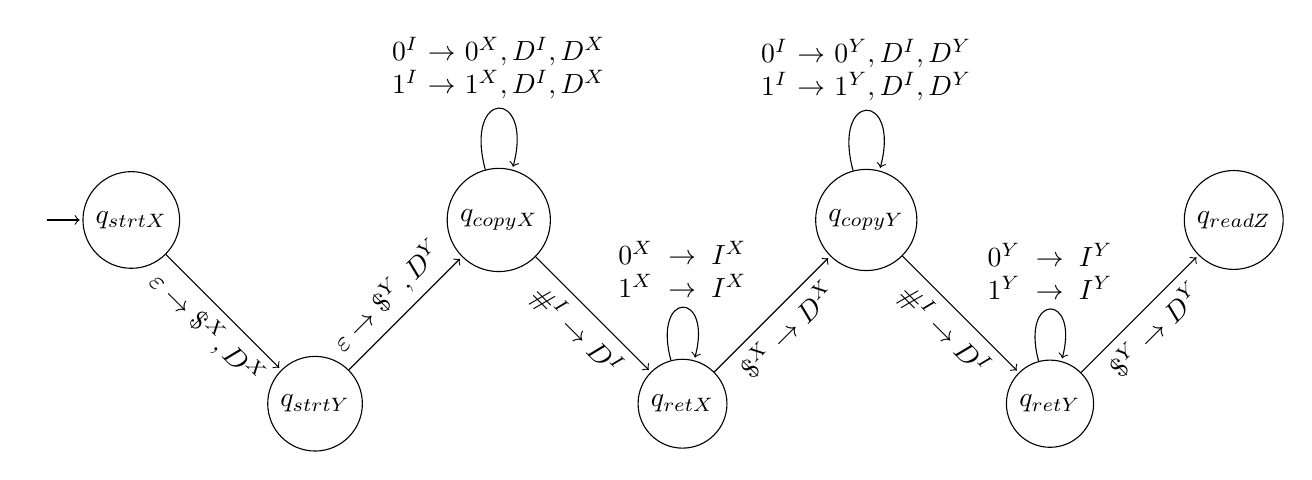
\begin{tikzpicture}[shorten >=1pt,node distance=3.3cm,on grid,auto]
\node[state,initial, initial text={}]	(q_00)											{$q_{strtX}$};
\node[state]							(q_01)		[below right=of q_00]				{$q_{strtY}$};
\node[state]							(q_1)		[above right=of q_01]				{$q_{copyX}$}; 
\node[state]							(q_2)		[below right=of q_1]				{$q_{retX}$}; 
\node[state]							(q_3)		[above right=of q_2]				{$q_{copyY}$}; 
\node[state]							(q_4)		[below right=of q_3]				{$q_{retY}$}; 
\node[state]							(q_f)		[above right=of q_4]				{$q_{readZ}$}; 
\path[->] 
(q_00)		edge					node[sloped, anchor=center, below]					{$\e \ra \$^X,D^X$}									(q_01)

(q_01)		edge					node[sloped, anchor=center, above]					{$\e \ra \$^Y,D^Y$}									(q_1)

(q_1)		edge	[loop above]	node[text width=3cm, align=center]					{$0^I \ra 0^X,D^I,D^X$\\$1^I \ra 1^X,D^I,D^X$}		()		
			edge					node[sloped, anchor=center, below]					{$\#^I \ra D^I$}									(q_2)

(q_2)		edge	[loop above]	node[text width=3cm, align=center]					{$0^X \ra I^X$\\$1^X \ra I^X$}						()		
			edge					node[sloped, anchor=center, below]					{$\$^X \ra D^X$}									(q_3)

(q_3)		edge	[loop above]	node[text width=3cm, align=center]					{$0^I \ra 0^Y,D^I,D^Y$\\$1^I \ra 1^Y,D^I,D^Y$}		()		
			edge					node[sloped, anchor=center, below]					{$\#^I \ra D^I$}									(q_4)

(q_4)		edge	[loop above]	node[text width=3cm, align=center]					{$0^Y \ra I^Y$\\$1^Y \ra I^Y$}						()		
			edge					node[sloped, anchor=center, below]					{$\$^Y \ra D^Y$}									(q_f)
;
\end{tikzpicture}
\end{center}
La etapa de procesamiento para $z$, por presentación, ha sido modificada para excluir las transiciones de rechazo. Éstas se pueden inferir como todas las transiciones que no estén explícitamente graficadas.
\begin{center}
\begin{tikzpicture}[shorten >=1pt,node distance=3.3cm,on grid,auto]
\node[state]							(q)												{$q_{readZ}$};
\node[state]							(q_0)		[above right=of q]					{$q_{z_0}$};
\node[state]							(q_00)		[above right=of q_0]				{$q_{z_0, x_0}$};
\node[state]							(q_01)		[right=of q_0]						{$q_{z_0, x_1}$};
\node[state]							(q_1)		[below right=of q]					{$q_{z_1}$};
\node[state]							(q_10)		[below right=of q_1]				{$q_{z_1, x_0}$}; 
\node[state]							(q_11)		[right=of q_1]						{$q_{z_1, x_1}$}; 
\node[state]							(q_u)		[left=of q]							{$q_{z_\sqcup}$}; 
\node[state]							(q_uu)		[left=of q_u]						{$q_{z_\sqcup, x_\sqcup}$}; 
\node[state,accepting]					(q_f)		[left=of q_uu]						{$q_{accept}$}; 
\path[->] 
(q)			edge					node[sloped, anchor=center, above]		{$0^I \ra D^I$}								(q_0)
			edge					node[sloped, anchor=center, above]		{$1^I \ra D^I$}								(q_1)
			edge					node[sloped, anchor=center, above]		{$\sqcup^I \ra D^I$}						(q_u)
			
(q_0)		edge					node[sloped, anchor=center, above]		{$0^X \ra D^X$}								(q_00)
			edge					node[sloped, anchor=center, above]		{$1^X \ra D^X$}								(q_01)
			
(q_00)		edge[bend right]		node[sloped, anchor=center, above]		{$1^Y \ra D^Y$}								(q)

(q_01)		edge					node[sloped, anchor=center, above]		{$0^Y \ra D^Y$}								(q)

(q_1)		edge					node[sloped, anchor=center, above]		{$0^X \ra D^X$}								(q_10)
			edge					node[sloped, anchor=center, above]		{$1^X \ra D^X$}								(q_11)
			
(q_10)		edge[bend left]			node[sloped, anchor=center, above]		{$0^Y \ra D^Y$}								(q)

(q_11)		edge					node[sloped, anchor=center, above]		{$1^Y \ra D^Y$}								(q)

(q_u)		edge					node[sloped, anchor=center, above]		{$\sqcup^X \ra D^X$}						(q_uu)
(q_uu)		edge					node[sloped, anchor=center, above]		{$\sqcup^Y \ra D^Y$}						(q_f)	
;
\end{tikzpicture}
\end{center}


\end{document}
